\thispagestyle{plain}
\color{red}
{\large \bf \underline {Instructions (remove these after completing your report ):}}
%\subsection{Edit and generate pdf}
\color{black}
\begin{enumerate}[label=\roman*.]
\item 	Double-click in the page header and replace “Project Name” text with your short project name.

\item \textcolor{blue} {
{If you have an external guide, ensure to insert (Signature of External Guide) at the left of (Signature of the External Examiner) on the APPROVAL page.}} If inserted, ensure to align the second line with the first line.

\item Insert \textbf{Appendix section(s)} at the end of this document if you need to elaborate any specific item, e.g. Data Collection if it is taking too many pages to cover.

\item 	\textcolor{blue}{\textbf{At the time of final examination, 1 spiral-bound project report should be submitted to the department in addition to the soft copy deliverables}}.

\item Citations should be used for all referred texts using appropriate numbers within square bracket for all mapped references under \textbf{References} section. You should check any standard journal paper for typical use of citations. 

\item 	Select Content (TOC), and apply Font Size=12. After completing the document, ensure to right-click on ToC $\rightarrow$ Update field  $\rightarrow$ Update entire table for automatically updating the index. If needed, change the font or adjust headings so that TOC can be fitted in a single page.

\item	Except under TOC, \textbf{Font} Style=”Times New Roman”, Font Size=”12” and Alignment=”Justified” should be uniformly used for the project documentation. Needless to say \textbf{spellchecker} should be used. 

\item Team should perform reasonable numbers of \textbf{proof reading} for avoiding unintentional errors and factual discrepancies before appearing in project viva.

\item	For all \textbf{ figures}, captions should be bold with centrally aligned and should be positioned below the figures, e.g.

Using MS-Word features, insert figures and tables after they are cited in the text so that they can automatically come after inserting / updating TOC.	 

Use a text box to insert a graphic (which is ideally a 300 dpi TIFF or EPS file, with all fonts embedded) because, in an MS Word document, this method is somewhat more stable than directly inserting a picture.

To have non-visible rules on your frame, use the MSWord “Format” pull-down menu, select Text Box $>$ Colors and Lines to choose No Fill and No Line.

\item For all \textbf{tables}, captions should be bold with centrally aligned and should be positioned above the tables, e.g.
\begin{figure}[h]  % Optional: figure environment to allow caption and positioning
    \centering      % Center the image
    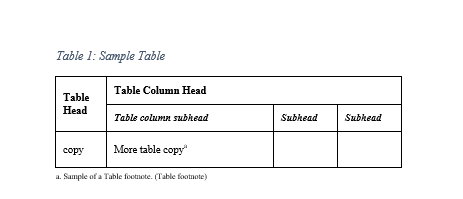
\includegraphics[width=\textwidth]{Table} % Specify the image file name
    %\caption{A caption for the image.}  % Optional: add a caption
    \label{fig:example}  % Optional: label for referencing the image
\end{figure}


\item	Based on your unique project, sections can be slightly altered over this generic template.

\end{enumerate}
\begin{comment}
    

\begin{enumerate}
\item You need to create an account in overleaf \url{https://www.overleaf.com/project} (if not already created) and login.
\item Select `New project' $\rightarrow$ `Upload project'  $\rightarrow$ select `LaTex\_template\_BTP\_Report.zip' file.
You need to do this step only once.
Next time on-wards, you can directly access the folder in overleaf and make necessary changes.
\item Only one person from the group can upload the project and the share the link to other members of the group who can edit and view the report.
\item Once the folder is loaded, select `BTP\_report.tex' file and click the `Recompile' option. On the right window, you can see the generated pdf where the {\LaTeX} source code is available on the left window.
\item In the `BTP\_report.tex' file change
\begin{itemize}
    \item Project title 
    \item Supervisor name
    \item Supervisor designation 
    \item Name of the HOD
    \item Designation of the HOD 
\item Names and roll numbers of the students
\end{itemize}
\item `Recompile' again to check if the changes are reflected.
\item The PDF file can also be downloaded.
\end{enumerate}
%%\subsection{Adding citations, tables, figures, equations}
\begin{description}
\item \textbf{Equations:}
Basic equations can be written using  Inline math modes such as
\begin{itemize}
    \item using \verb|\(...\)|: \verb|\(x^2 + y^2 = z^2\)| will generate \(x^2 + y^2 = z^2\)
    \item using \texttt{\$...\$}:  \verb|$(x^2 + y^2 = z^2)$| will generate  $(x^2 + y^2 = z^2)$
    \item or, using \verb|\begin{math}...\end{math}|: \\ \verb|\begin{math} x^2 + y^2 = z^2 \end{math}| will generate   \begin{math}(x^2 + y^2 = z^2)\end{math}
\end{itemize}
You can use \verb|\begin{equation}...\end{equation}| for display modes such as 
\verb|\begin{equation} x^2 + y^2 = z^2 \end{equation}| resulting to
\begin{equation} x^2 + y^2 = z^2 \end{equation}
Other details such as adding subscript, superscript, fractions, you can refer to \url{https://www.overleaf.com/learn/latex/Mathematical_expressions}
\item \textbf{Citations:} The citations should be made through adding a `BibTex' entry in `references.bib' file.
Check the examples below:
\begin{verbatim}
  @Article{Einstein,
  author =       "Albert Einstein",
  title =        "{Zur Elektrodynamik bewegter K{\"o}rper}. ({German})
                 [{On} the electrodynamics of moving bodies]",
  journal =      "Annalen der Physik",
  volume =       "322",
  number =       "10",
  pages =        "891--921",
  year =         "1905",
  DOI =          "http://dx.doi.org/10.1002/andp.19053221004"
} 
@online{WinNT,
  author = {MultiMedia LLC},
  title = {{MS Windows NT} Kernel Description},
  year = 1999,
  url = {http://web.archive.org/web/20080207010024},
  urldate = {2010-09-30}
}

@book{knuth1984texbook,
  title={The texbook},
  author={Knuth, Donald Ervin and Bibby, Duane},
  volume={15},
  year={1984},
  publisher={Addison-Wesley Reading}
}  
\end{verbatim}

    % Reference to text book of Donald Knuth \cite{knuth_texboo k}.
\url{https://www.overleaf.com/learn/latex/Bibliography_management_with_bibtex}
Template entries for `BibTex' types of article, conference, book, thesis can be found here \url{https://www.bibtex.com/format/#templates}

The formatted `BibTex' entries of a reference material can also be found in Google Scholar. Search with the title of the paper/thesis/book in Google scholar $\rightarrow$ Select `Cite' option at the bottom the search results $\rightarrow$ Select `Bibtex' option and copy the entry in `references.bib' file.
    


For more detailed examples refer to \url{https://www.overleaf.com/learn/latex/Tables}

\end{description}
{\bf Important}
\begin{enumerate}
\item \textcolor{red}{Remove (Signature of External Guide, if applicable) on the \textbf{CERTIFICATE} page if you don't have an external guide. In any case, \textbf{(Signature of the External Examiner) must be right aligned} as in the template.}
  \item For avoiding plagiarism, citations should be used for all referred texts using appropriate numbers within square bracket for all mapped references under Section 8: References. You should check any standard journal paper for typical use of citations. 

  \item  \textcolor{red}{\textbf{Change the page header and replace “Project Name” text with your short project name}}.


    \item Select the document class 12pt. 

\item Team should perform reasonable numbers of proof reading for avoiding unintentional errors and factual discrepancies before appearing in project viva.


\item  At the time of final examination, (n+1) hard-bound copies of the report requiring (n+1) letter heads should be submitted, where n = team-size and 1 copy should be reserved for the department (not applicable for Midterm or Checkpoint Review)

\item For all figures, captions should be bold with centrally aligned and should be positioned below the figures, e.g.
All image files are to be stored in the Images folder.
For all figures, captions should be bold with centrally aligned and should be
positioned below the figures.
One such example is shown below:
\begin{verbatim}
  \begin{figure}[ht]
    \centering
    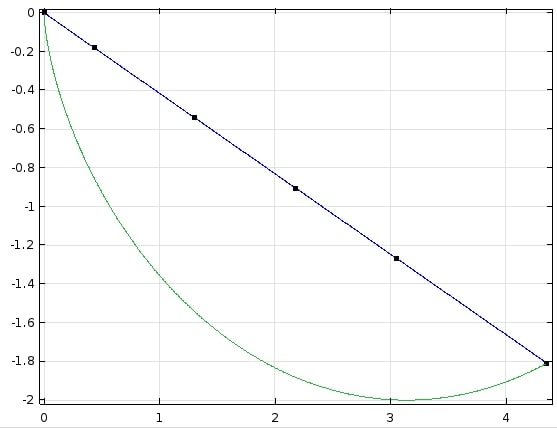
\includegraphics[width=0.5\textwidth]{Brachistochrone-curve-plot.jpg}
    \caption{Sample Image}
    \label{fig:1a}
\end{figure}  
\end{verbatim}
\begin{figure}[ht]
    \centering
    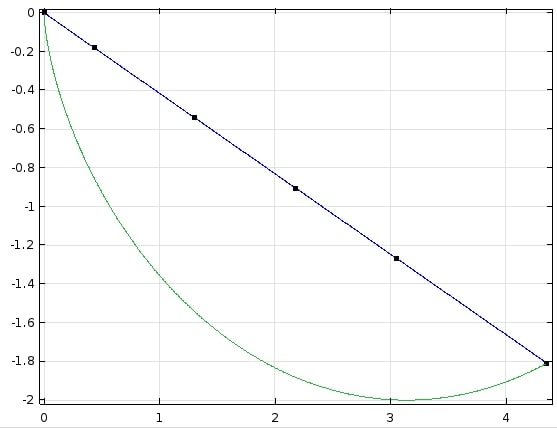
\includegraphics[width=0.5\textwidth]{Brachistochrone-curve-plot.jpg}
    \caption{Sample Image}
    \label{fig:1a}
\end{figure}
This figure will be referenced in the text as Figure \ref{fig:1a}.
For more detailed references for adding figures, refer to \url{https://www.overleaf.com/learn/latex/Inserting_Images}.

\item 
For all tables, captions should be bold with centrally aligned and should be positioned above the tables.
One such example is shown here. 
\begin{verbatim}
\begin{table}[h!]
  \begin{center}
    \caption{Your first table with 3 columns and 5 rows}
    \label{tab:table1}
    
    \begin{tabular}{|c|r|l|} % <-- Alignments: 1st column middle, 
    % 2nd right and 3rd left, 
    % with vertical lines in between each column and row
    % \\
    \hline
      \textbf{Value 1} & \textbf{Value 2} & \textbf{Value 3}\\
      $\alpha$ & $\beta$ & $\gamma$ \\
      \hline
      1 & 1110.1 & a\\
      2 & 10.1 & b\\
      3 & 23.113231 & c\\
      \hline
    \end{tabular}
  \end{center}
\end{table}
\end{verbatim}
\begin{table}[h!]
  \begin{center}
    \caption{Your first table with 3 columns and 5 rows}
    \label{tab:table1}
    
    \begin{tabular}{|c|r|l|} % <-- Alignments: 1st column middle, 2nd right and 3rd left, with vertical lines in between each column and row
    % \\
    \hline
      \textbf{Value 1} & \textbf{Value 2} & \textbf{Value 3}\\
      $\alpha$ & $\beta$ & $\gamma$ \\
      \hline
      1 & 1110.1 & a\\
      2 & 10.1 & b\\
      3 & 23.113231 & c\\
      \hline
    \end{tabular}
  \end{center}
\end{table}

This table can be referenced in the text as Table \ref{tab:table1}.

For more detailed examples refer to \url{https://www.overleaf.com/learn/latex/Tables}

\item If you have published related paper(s) in a standard journal / presented in a recognized conference, please ensure to refer the same under Section 8: References as well as including communication on your paper(s) acceptance / publishing note under the Appendix section. You should also show appropriate documentation at the time of project viva.
\item Depending on the type of your project, sections can be altered to this generic template.



\end{enumerate}

\end{comment}
